\section{Attritable MCTS with Regret Minimization}
% \GR{introduce to the section: what does it contain? We first prove the root cause of the inefficiency of existing decentralized MCTS approaches (without reset). Then we draw inspiration for designing our new approach, still based on a  decentralized version of MCTS.} 

In this section, we first give a brief introduction to Monte Carlo Tree Search and its most popular decentralized version. We then show the root cause of the inefficiency of existing decentralized MCTS approaches with attrition. 
% Finally, we present our A-MCTS algorithm as a solution to the multi-agent planning in attrition settings problem \ref{prob:1}.


% \subsection{Why does Decentralized MCTS fail with attrition?}
MCTS is an excellent approach for online planning problems \citep{kocsis2006improved}. The tree $\mathcal{T}_n$ for agent $n$ is defined such that each node $s$ of the tree represents a state and each edge $a$ starting from that node represents an available action. A branch from the root node to another node represents a valid action sequence. The tree is incrementally grown via a four-step process: \emph{selection}, \emph{expansion}, \emph{rollout}, and \emph{backpropagation}. Decentralized Monte Carlo Tree Search (Dec-MCTS)~\citep{best2019dec} extends the power of MCTS to MAS using intention sharing. Specifically, agent $n$ maintains a probability mass function $q_n(x_n)$ over the set of all possible action sequences $\Xc_n$, where $x_n \in \Xc_n$ is a primitive action sequence. The intentions of other agents except agent $n$ are denoted by $q_{-n}$ and $\Xc_{-n}$. By taking a probabilistic sampling from the communicated intention, each agent can reconstruct the global utility. To create better coordination, rather than optimizing directly for the global utility $U_g$ of the entire team, each agent $n$ instead optimizes for a local \emph{marginal contribution} utility function $U_n$. That is, agent $n$ estimates the rollout score for executing $x_n$ as: 
\begin{equation} 
\label{eq:marginal}
     F_n(x_n) = U_n(x_n, x_{-n}) = U_g(x_n, x_{-n}) - U_g(x_{-n})\ ,
\end{equation}
where $U_g(x_{-n})$ is the global utility without the contribution of agent $n$.
% \subsection{Dec-MCTS Under Failures}
% \GR{make the paper more general, not just comparing with DEC MCTS. How can we still retain this section without reducing it to a comment on the drawbacks of DEC MCTS? Can we cast this section as a more general statement about a problem with attrition arising when submodularity is there?}

We now analyze Dec-MCTS asymptotic behavior when agents fail. We are particularly interested in \textit{submodular} reward functions, frequently arising in data collection problems~\citep{corah2017efficient,satsangi2018exploiting}. Submodular set function, which is defined in Definition~\ref{def:submodular}, satisfies the diminishing returns property. Regarding the information-gathering problem discussed in this paper (see Section~\ref{sec:problem_formulation}), the marginal gain of adding a new location to the set of visited locations decreases as the number of locations visited increases.

\begin{definition}[Submodular set function]
    \label{def:submodular}
    Let $g: 2^\Omega \rightarrow \mathbb{R}$ be a set function where $2^\Omega$ is the power set of $\Omega$. Then \emph{g} is a submodular function if for every $X, Y \subseteq \Omega$ with $X \subseteq Y$ and every $x \in \Omega \setminus Y$ the following inequality holds
    $$g(X \cup x) - g(X) \ge  g(Y \cup x) - g(Y)\ .$$
\end{definition}

% https://www.sciencedirect.com/science/article/pii/S0005109819301281
In particular, at iteration $t$, let $x_n$ denote the chosen action sequence of agent $n$ and $x_{-n}$ denote the combined sampled action sequences of other agents. Assume that at the next iteration $t+1$, a subset of agents fails. Let $x^\prime_{-n}$ be the combined sampled action sequences of all agents except agent $n$ and the lost agents (i.e., that is $x^\prime_{-n} \subseteq x_{-n}$).

\begin{proposition}
\label{prop:nondecreasingreward}
If the global objective function $U_g$ is submodular, then $
    F_n^{(t+1)}(x^*_n) \ge F_n^{(t)}(x^*_n)$ by the diminishing return property due to submodularity, where $F_n(x_n)$ is defined in (\ref{eq:marginal}).
\end{proposition}

\begin{figure*}[!ht]
	\begin{center}
 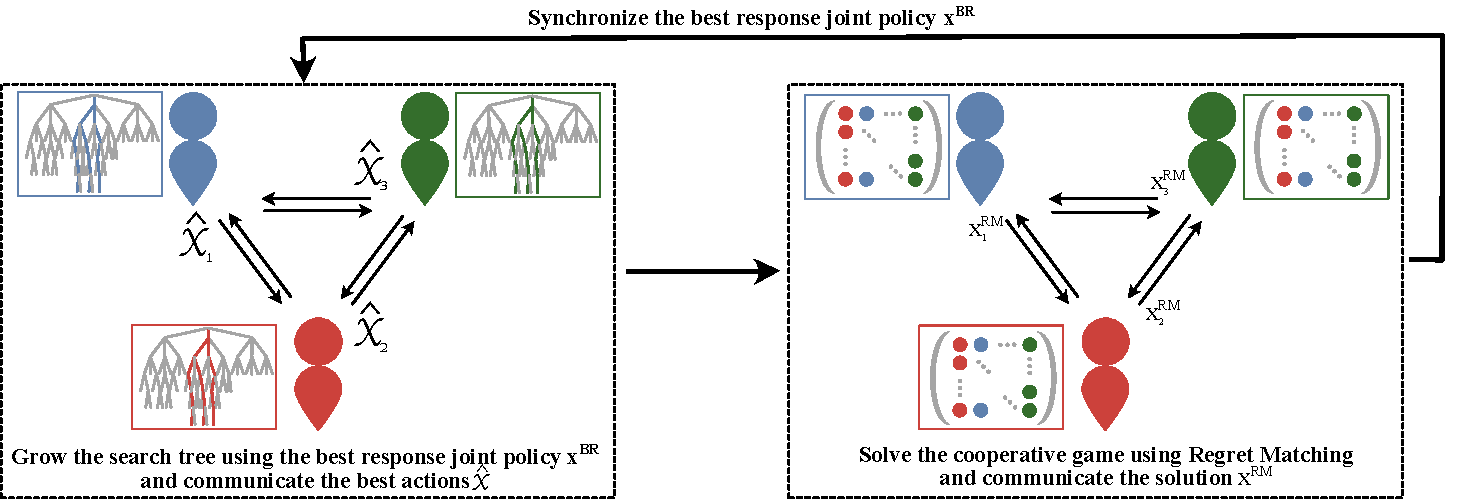
\includegraphics[width=0.7\linewidth]{figs/algo.pdf}
		\caption{\footnotesize Overview of the A-MCTS algorithm. Agents incrementally grow the search using the best response policy $x^{BR}$ and communicate their best actions $\hat{\mathcal{X}}$. Regret Matching is then used to compute distributively a joint policy for the cooperative game. These solutions are synchronized and the most payoff-dominant is chosen as the best response policy $x^{BR}$.
        \label{fig:algo}}
	\end{center}
\end{figure*}

Proposition~\ref{prop:nondecreasingreward} states that if some agents fail during the mission, the remaining agents would mistakenly perceive that the contribution of their previous actions increases. Hence, they would not be aware of the actual reduction of the global utility and update their plans\footnote{For analysis of Dec-MCTS behavior when agent failures occur after the algorithm has converged, please see Appendix A in the Supplementary Material}. Fixing this issue requires both a new, context-aware way to compute the reward and a new way to coordinate the actions with other agents on this new reward function. In the next section, we present our proposed algorithm for the multi-agent planning in attrition settings problem \ref{prob:1}.
